\documentclass[svgnames]{uvamscse} %Add xcolor parameter here to prevent conflict.

\usepackage[utf8]{inputenc}
\usepackage[english]{babel}
\usepackage{booktabs}
\usepackage{array}
\usepackage{paralist}
\usepackage{longtable}
\usepackage{amsmath,amssymb,amsthm}
\usepackage{csquotes}
\usepackage{xcolor}
\usepackage{framed}
\usepackage{listings}
\usepackage{protobuf/lang}  % include language definition for protobuf
\usepackage{protobuf/style} % include custom style for proto declarations.
\usepackage[backend=biber,style=numeric]{biblatex}
\usepackage[colorinlistoftodos]{todonotes}
\usepackage{pgfgantt}
\usepackage{hyperref}
\usepackage[toc,acronym,nogroupskip,nohypertypes={acronym}]{glossaries}
\usepackage{subcaption}
\hypersetup{pdfstartview={XYZ null null null}}
\colorlet{shadecolor}{yellow}

%Title page
\title{Improving management of virtual container networks on DC/OS}
\author{Willem Jan Glerum - 11317493}
\authemail{wjglerum@gmail.com}
\host{Lunatech Labs B.V. \url{https://lunatech.com} }
\supervisor{dr. Paola Grosso \url{p.grosso@uva.nl}}
\hostsupervisor{dr. Adrien Haxaire \url{adrien.haxaire@lunatech.nl}}
\date{\today}
%Random virtual network image
\coverpic[200pt]{images/virtual.png}

\abstract{
Developers use containers to deploy their applications highly available on container orchestration platforms. On Mesosphere DC/OS it is possible to isolate services with virtual container networks and network policies provided by CNI plugins. Isolation is often needed for privacy and security concerns and for separating different tenants on the platform. At the time of writing, there is no method in place to centrally manage virtual networks and network policies on DC/OS.

The goal of this thesis is to understand the current problems in managing virtual container networks on DC/OS and to propose solutions to these problems. To do this, the study first gives background information on the used technologies to be able to identify the current problems. Based on this study, a proof of concept is presented. It is able to centrally manage network policies for different vendors.

The solution proposed in this thesis shows that it is possible to improve the management of virtual networks without a radical change in the architecture of DC/OS. Operators are now able to retrieve the current state of applied network policies and adjust them as needed.
}

%This section summarises the content of the thesis for potential readers who do not have time to read it whole,  or for those undecided whether to read it at all. Sum up the following aspects:
%    \item relevance and motivation for the research
%    \item research questions and a brief description of the research method
%    \item results, contributions and conclusions

%Styles for the lstlisting blocks.
%\input{lststyles}

%Glossary register:
\newacronym{cni}{CNI}{Container Network Interface}
\newacronym{sdn}{SDN}{Software Defined Networking}
\newacronym{poc}{PoC}{Proof of Concept}
\newacronym{ucr}{UCR}{Universal Container Runtime}
\newacronym{iot}{IoT}{Internet of Things}
\newacronym{dcos}{DC/OS}{The Datacenter Operating System}
\newacronym{vm}{VM}{Virtual Machine}
\newacronym{os}{OS}{Operating System}
\newacronym{aws}{AWS}{Amazon Web Services}
\newacronym{gcp}{GCP}{Google Cloud Platform}
\newacronym{ipam}{IPAM}{IP Address Management}
\newacronym{api}{API}{Application Programming Interface}
\newacronym{http}{HTTP}{Hypertext Transfer Protocol}
\newacronym{grpc}{gRPC}{gRPC Remote Procedure Calls}
\newacronym{bpf}{BPF}{Berkeley Packet Filter}
\newacronym{jit}{JIT}{Just In Time}
\newacronym{bgp}{BGP}{Border Gateway Protocol}
\newacronym{bird}{BIRD}{BIRD Internet Routing Daemon}
\newacronym{nat}{NAT}{Network Address Translation}
\newacronym{ip}{IP address}{Internet Protocol address}
\newacronym{dhcp}{DHCP}{Dynamic Host Configuration Protocol}
\newacronym{vlan}{VLAN}{Virtual LAN}
\newacronym{cgroup}{cgroup}{Control Group}
\newacronym{vxlan}{VXLAN}{Virtual Extensible LAN}

\makeglossaries

%Bibliography DB
\addbibresource{refs.bib}

%Useful definitions for (long)tables:
\newcolumntype{L}[1]{>{\raggedright\let\newline\\\arraybackslash\hspace{0pt}}p{#1}}
\newcolumntype{C}[1]{>{\centering\let\newline\\\arraybackslash\hspace{0pt}}p{#1}}
\newcolumntype{R}[1]{>{\raggedleft\let\newline\\\arraybackslash\hspace{0pt}}p{#1}}

\begin{document}

\maketitle
\chapter{Introduction}
\label{chap:introduction}

\chapter{Background and context}
\emph{This chapter contains all the information needed to put the thesis into
context. It is common to use a revised version of your literature survey for this purpose. It
is important to explicitly refer from your text to sources you have used, they will be listed in
your bibliography.}
\chapter{Research}
%\emph{This chapter reports on the execution of the research method as described in an earlier chapter. If the research has been divided into phases, they are introduced, reported on and concluded individually. If needed, this chapter could be split up to balance out the sizes of all chapters.}
This chapter reports on the execution of the research to demonstrate what has been done. First we explain the current difficulties with managing virtual networks on \gls{dcos}. Next we explore the approach how another popular container orchestration platform, Kubernetes, handles virtual networks. Last we explain the approach we took to build the \gls{poc}.

\section{Current state of virtual networks in DC/OS}
\Gls{dcos} provides virtual networks by itself as overlay networks which can be used by the Docker and Mesos containerizer. This overlay is prepacked and enabled by default on the cluster. \Gls{cni} plugins are also supported on \gls{dcos} and can be used by both containerizers.

\subsection{DC/OS virutal networks}
The overlay network was introduced to enable an IP-per-container model in \gls{dcos}. This allows operators to run applications on the default ports without worrying about port conflicts. This is done by creating an overlay network using \gls{vxlan}\cite{mahalingam2014virtual} which is supported by the Linux kernel. It works by creating two network bridges on each host, one for each containerizer. Containers on the same host and bridge can communicate directly with each other over the network bridge. And a packet from a Mesos container to a Docker container will be routed through both bridges. A packet from a Mesos container on Agent~1 to a Docker container on Agent~2 follows a different path. First the packet will be routed to the Mesos bridge, the host's network stack consumes the package and encapsulates using \gls{vxlan} on Agent~1. Next Agent~2 decapsulates this packet and sends it up to the Docker bridge to be sent to the Docker container as can be seen in Figure~\ref{fig:dcos-overlay-arch}.

IP address are managed by the agent itself instead of a central location. A central location requires a reliably and consistent way of handing IP addresses in the cluster. The default configuration uses a \texttt{9.0.0.0/8} subnet, this will devided in smaller chunks, a \texttt{/24} to be managed by every agent itself. On the agent this subnet is divided into two equal subnets for each containerizer, resulting in 32 usable IP addresses for each container type on every agent.
\begin{figure}
    \centering
    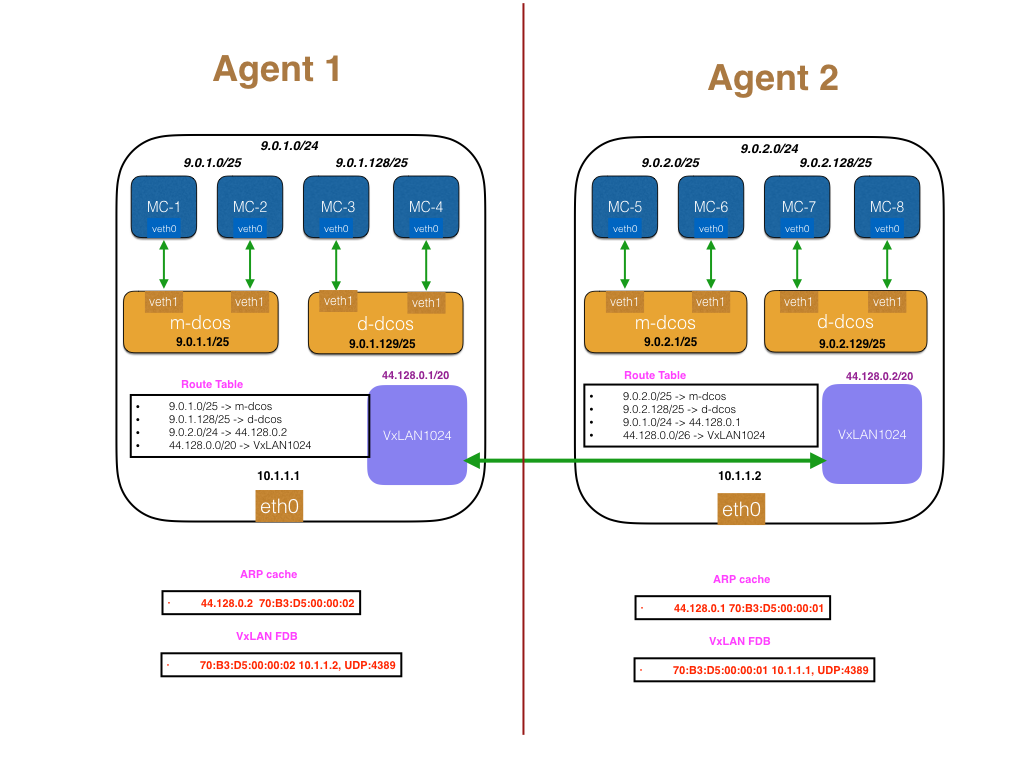
\includegraphics[width=1\columnwidth]{images/dcos-overlay-arch}
    \caption{DC/OS overlay in action\cite{dcos_overlay_arch}}
    \label{fig:dcos-overlay-arch}
\end{figure}

The default overlay network has the following limitations:
\begin{itemize}
    \item A limit on the number of usable IP addresses on each host, determined by the network prefix size. The default maximum is 32 Mesos and 32 Docker containers.
    \item Only IPv6 support for Docker containers, Mesos containers will fail to start.
    \item Operators are only able to create virtual networks during installation, this requires planning on before hand.
    \item The length of network names is limited as the Linux kernel only allows 15 characters for a network interface name.
    \item Marathon cannot execute healhtchecks in the default configurations as Marathon itself is not running on the virtual network.
\end{itemize}

\subsection{CNI plugins on DC/OS}
Too allow for more flexibility with virtual networks operators can also chose to create network with other providers.
\begin{displayquote}
    ``NOTE: The network tab currently displays information about containers that are associated with virtual networks managed by DC/OS overlay. It does not have information about containers running on virtual networks managed by any other CNI/CNM provider.'' %https://docs.mesosphere.com/1.11/networking/SDN/dcos-overlay/#limitations
\end{displayquote}



\subsection{Problems}

\section{Virtual networks in Kubernetes}

\section{Proof of concept}

\chapter{Proof of Concept}
\label{chap:proof-of-concept}
%\emph{This chapter presents and clarifies the results obtained during the research. The focus should be on the factual results, not the interpretation or discussion. Tables and graphics should be used to increase the clarity of the results where applicable.}
In Chapter~\ref{chap:research} we explained the difficulties of managing virtual network on \gls{dcos}. The main problem is that operators of clusters cannot get an overview of the virtual networks and the applied network policies. In this chapter we propose two solutions. First we explain how we could do this by expanding the \gls{cni} specification, next we report on the solution we implemented in the \gls{poc}. \todo[inline]{Rephrase as this is not properly linked to previous chapter}

\section{Extending CNI}
\label{sec:expanding-cni}
\todo[inline]{vague/confusing/rewrite}
One of the first ideas we had was to extend \gls{cni} to be bi-directional which would allow operators to retrieve information about the virtual networks, to see which virtual networks are present and which containers are connected to the virtual network. The specification already has an \texttt{ADD} action that returns the network state of a container when it has been created. However this does not allow to query the current state of the networks. It would require to create a custom solution to keep track of the current network state and follow the changes to the containers. To make this work we would have to adapt the \gls{cni} specification to include a new action to allow querying of the network state of containers. This new action could logically be called \texttt{GET}, returning the same information when the \texttt{ADD} action was invoked and allows for caching of the results.

We decided not to touch the \gls{cni} specification for this thesis, as creating a new action in the \gls{cni} specification would require coordination and working together with different people and companies developing \gls{cni} plugins. At the beginning of this thesis the community was already discussing the need for a new action that would retrieve the current state of the network of a container. Maintainers did not agree yet on whether this should be implemented. Not only would we have to adjust the specification, we would also have to extend the \gls{cni} plugins in use at the client to support a new action. Furthermore this action will only expose information about the network state of the container, not the state of the virtual networks in the cluster which operators want to see. Network policies are not included in the \gls{cni} specification. With the new \texttt{GET} action in place we would still need a different solution for managing network policies. 

\section{Network Object API}
\label{sec:networkobject-api}
Instead of extending the \gls{cni} specification we decided to build a \gls{poc} for a new system in \gls{dcos}. A central \gls{api} for managing virtual container network related components in \gls{dcos}. We introduce a network object model. In this model an operator can define a network object with the relevant configuration for a network. First we explain the model in Section~\ref{subsec:network-object-model}, next the global system design and features in Section~\ref{subsec:system-design} and we conclude with the implemented \gls{poc} in Section~\ref{subsec:poc-architecture}.

\subsection{Network Object Model}
\label{subsec:network-object-model}
The network object model contains different properties for defining networks in \gls{dcos}. The specification for this model can be found in Listing~\ref{lst:nom}. We explain the basic idea for each component.

\lstinputlisting[label={lst:nom},caption={Network Object Model in Protocol buffers format},language=protobuf2,style=protobuf]{code/networkobject.proto}

\begin{itemize}
    \item[\textbf{Virtual Network}] Specifies the basic properties of a network. Containing the name and subnet of a virtual network.
    \item[\textbf{Network Driver}] Driver for the specified network, which can be  a \gls{dcos} overlay network, a standard plugin, or a \gls{cni} plugin.
    \item[\textbf{Security Policy}] A set of firewall rules for a given network. These rules can be either level 4 rules for packet filtering based on port and host or level 7 rules to inspect on application level. Rules can also be applied based on labels to firewall specific applications or traffic.
    \item[\textbf{Network Service}] Services could be a set of different things to attach to a network. For example a cloud provider integration for ingress traffic to the cluster.
\end{itemize}

\subsection{Overall System Design}
\label{subsec:system-design}
The idea is that this new service runs on the masters of a \gls{dcos} cluster. We choose the masters as they are already highly-available in a default setup. Both CockroachDB\cite{cockroachdb} and Zookeeper\cite{zookeeper} are already running on the master providing distributed storage for other \gls{dcos} components. It is also possible to use etcd\cite{etcd} as a central key-value store on the master. However this decision is out of scope for this thesis as the \gls{poc} in Section~\ref{subsec:poc-architecture} uses a different approach.

The system is based on the idea of the kube-apiserver from Kubernetes as discussed in Section~\ref{subsec:kubernetes} where an operator can query the current state and submit the required state. The system would not only provide insight to the available virtual networks and policies, but also be open for example to integrate with cloud providers for North-South traffic into the cluster. The new system should have the following features: \todo[inline]{create diagram of system design}
\begin{itemize}
    \item Run highly-available on the masters
    \item Use a distributed higly-available storage solution
    \item Show an overview of the available virtual networks
    \item Allow to create, configure and delete virtual networks
    \item Give an overview of the applied network policies per network, tasks or framework.
    \item Allow to create, configure and delete network policies
    \item Integrate with cloud providers to configure ingress traffic
\end{itemize}

\subsection{PoC Architecture}
\label{subsec:poc-architecture}
We want to show a basic \gls{poc} \todo[inline]{Explain basic, not all functions} where an operator can see the configured policies for a given container on a virtual network. Showing the available networks can be easily achieved with this new API in place, however creating virtual networks is more difficult. To create a virtual network on demand we would have to distribute the plugin and its configuration to every node, requiring a custom build solution. Mesoshpere is working on providing such a system to distribute files to nodes for volume mount, which we could later use to distribute network specific files to every node.

We also reused parts from the opensource project Kubernetes to save time. Mesosphere recently added support for running Kubernetes on a \gls{dcos} cluster. We reuse the kube-apiserver with \glspl{crd} to submit and query network objects to be stored in etcd. This saves us from the burden of writing our own REST API server and setting it up manually on the masters. The kube-apiserver runs as a single container however it depends on other Kubernetes components such as etcd to store information. Instead of trying to strip the kube-apiserver from Kubernetes components, we run an entire Kubernetes cluster on our \gls{dcos} cluster. This does cause some overhead, but we are still able to run a full cluster on a single Macbook Pro with 16GB of RAM. It did took some time to tune the CPU and memory usage to allow it to run on a single developer machine. For a production ready solution we should implement both the \gls{api} server and storage to run on the masters as discussed in Section~\ref{subsec:system-design}.

Next we created a custom controller written in GoLang\cite{golang} based on one of the examples provided by Kubernetes for dealing with \glspl{crd}. This controller listens to the updates on the kube-apiserver of a specific \gls{crd}. With a custom Dockerfile we can build a container and run it on the \gls{dcos} cluster. Connect it to the kube-apiserver, allowing us to rapidly prototype and try out new queries for our network objects. The only difficulty is getting the configuration and credentials for access to the Kubernetes cluster in our custom controller. Luckily Marathon has support for volume mounts, so we can generate the configuration file once on the host allowing the container to read it from the volume mount to connect to the Kubernetes cluster.

In short we use the following components for this \gls{poc}:
\begin{itemize}
    \item Kubernetes as a framework on \gls{dcos}
    \item Utilise the kube-apiserver with etcd to store our network object \gls{crd}
    \item Custom controller listening for events and integrates with the Calico \gls{api}
\end{itemize}
\todo[inline]{create poc architecture image}

\chapter{Validation of PoC}
\label{chap:validation}
\todo[inline]{Report on how the PoC answers RQ2 and addresses the issues RQ1}

\chapter{Conclusions}
\label{chap:conclusions}
%\emph{This chapter contains the analysis and interpretation of the results. The research questions are answered as best as possible with the results that were obtained. The analysis also discussed parts of the questions that were left unanswered. An important topic is the validity of the results. What methods of validation were used? Could the results be generalised to other cases? What threats to validity can be identified? There is room here to discuss the results of related scientific literature here as well. How do the results obtained here relate to other work, and what consequences are there? Did your approach work better or worse? Did you learn anything new compared to the already existing body of knowledge? Finally, what could you say in hindsight on the research approach by followed? What could have done better? What lessons have been learned? What could other researchers use from your experience? A separate section should be devoted to future work", i.e., possible extension points of your work that you have identified. Even other researchers should be able to use those as a starting point.}
This thesis describes the difficulties in managing virtual networks on \gls{dcos}. For operators it is possible to create virtual networks using \gls{cni} plugins and some have support for network policies. However there is no central place in \gls{dcos} to see and configure those networks and policies. Unlike in Kubernetes where operators can manage the virtual networks by providing a desired state, the cluster then takes care of configuring the virtual networks and network policies. We first explored the different technologies in use and explained how they all work. This gives us a good foundation to be able to understand the difficulties in managing virtual container networks. Next we conducted a research on the features that are missing to manage those networks and how other vendors such as Kubernetes handle this.

Next a \gls{poc} was built to improve the management of virtual networks on \gls{dcos}. This \gls{poc} demonstrates that it is possible to abstract different \gls{sdn} solutions into one central \gls{api}. This \gls{api} can be used by operators to create new policies regardless of the plugins implemented within the cluster. Furthermore it enables developers to debug and see which policies are blocking traffic to their applications. Giving insight to developers deemed crucial as developers would end up removing their applications from the virtual network to make them work. This is an unwanted situation at Lunatech's automotive client because they need to isolate different parts of their data processing pipeline for privacy and security concerns. The newly built api-server is able to provide useful insights into the state of the network.

To conclude we can say that the new solution improves the management of virtual networks on \gls{dcos}. As operators and developers are able to retrieve and configure the virtual network state from a central place instead of having to dig into the concrete implementations of each \gls{sdn} provider.

\chapter{Future work}
\label{chap:future-work}
At the moment the \gls{poc} includes an entire Kubernetes cluster, so that's one obvious point of improvement towards a final solution. As future work we could implement our own api-server for the network objects and make it run highly available on all the masters in a \gls{dcos} cluster. Furthermore we need to extend the dcos-cli to include the new network objects that we have defined. Once this is in place we can extend the web interface of \gls{dcos} to query the api-server for network objects and display them in the web interface. This will help developers and operators to check which virtual networks are available and which network policies have been applied to their applications. In the future we could also create network diagrams to allow for inspection during a production problem or a security audit.

During this thesis we did not consider the creation of virtual networks from a central place as this was hard to achieve without a system that could distribute files to all agents. If such a system is in place we could make use of it to distribute the \gls{cni} plugins and their configuration files for the virtual networks, allowing developers to create new virtual networks using the custom controller that we implemented. Once the creation of virtual networks is implemented we can also provide the list of available virtual networks back to the users for them to select a network for their container.

Another extension could be a plugin model for cloud providers. At the moment operators need to manually configure load balancers as ingress points on a cloud platform to point to the right services, also called North-South traffic for a cluster. In the future we could create a plugin per cloud provider that automatically configures the load balancers, certificates and \gls{dns} records to point to the right services. We could also think of chaining different kind of plugins together. For example a plugin that logs all packets and another plugin that does traffic shaping of the same traffic.

We could also use the newly available information from the api-server to determine bottlenecks within clusters. When we have the list of current networks and policies we can leverage existing tools to monitor the network. Together with machine learning we could optimise traffic flows and apply the new network configuration using the same api-server. This could be a form of self adapting networks where we can ask the operator for confirmation or apply the new configuration automatically.


\clearpage

\addcontentsline{toc}{chapter}{Bibliography}
\printbibliography{}
\printglossaries

\appendix
\glsresetall 

\end{document}
